%%%%%%%%%%%%%%%%%%%%%%%%%%%%%%%%%%%%%
%Presentazione esame di Dottorato Davide Spataro
%introduction.tex
%Purpose: This file contains the introduction to the problem the thesis tries to solve, it shows why single chip performances are not improving as much as the moore's law predicts and introduces the concept of parallelism in computation and in numerical simulation.
%@author Davide Spataro
%@version 1.0 14/01/2018 Eindhoven
%%%%%%%%%%%%%%%%%%%%%%%%%%%%%%%%%%%%

%- La dimensione dei problemi che viene rislta oggigiorno è più grande. Il numero di applicazioni del calcolo scientifico sta aumentando con il numero di devices e di informazioni che la IoT sta fornendo. Questo implica che è richiesta una potenza di calcolo via via sempre maggiore
%
%- La potenza di calcolo aumentava fino a qualche anno fa in maniera esponenziale (mostra grafico) cioè raddoppiando il numero di transistor ogni anno. Ma questo trend non è più sostenibile per una serie di motivi (e ora che lavori in ASML te ne rendi ancora più conto). Dimensione dei transistor e calore per unita di superfice
%
%- Calcolo parallelo diventa fondamentale e negli ultimi 5 anni abbiamo visto un esplosione di parallelismo al punto che anche i telefoni sono macchine parallele con buone prestazioni. Fai esempio dei processori snapdragon.
%
%- Per cosa per esempio queste macchine nell'ambito del calcolo parallelo? risolvono equazioni differenziali etc. 
%Con che metodi lo fanno? molti, ma uno dei più usati è quello delle differenze finite. 
%
%Cosa fa questa tesi? 
 

\section{Motivations} 
\frame{\frametitle{Introduction and Motivations}
\centering
\begin{block}{}
	\centering 
\textbf{The amount of raw information available has increased dramatically during the last 10 years.}
	\begin{figure}
		\centering
			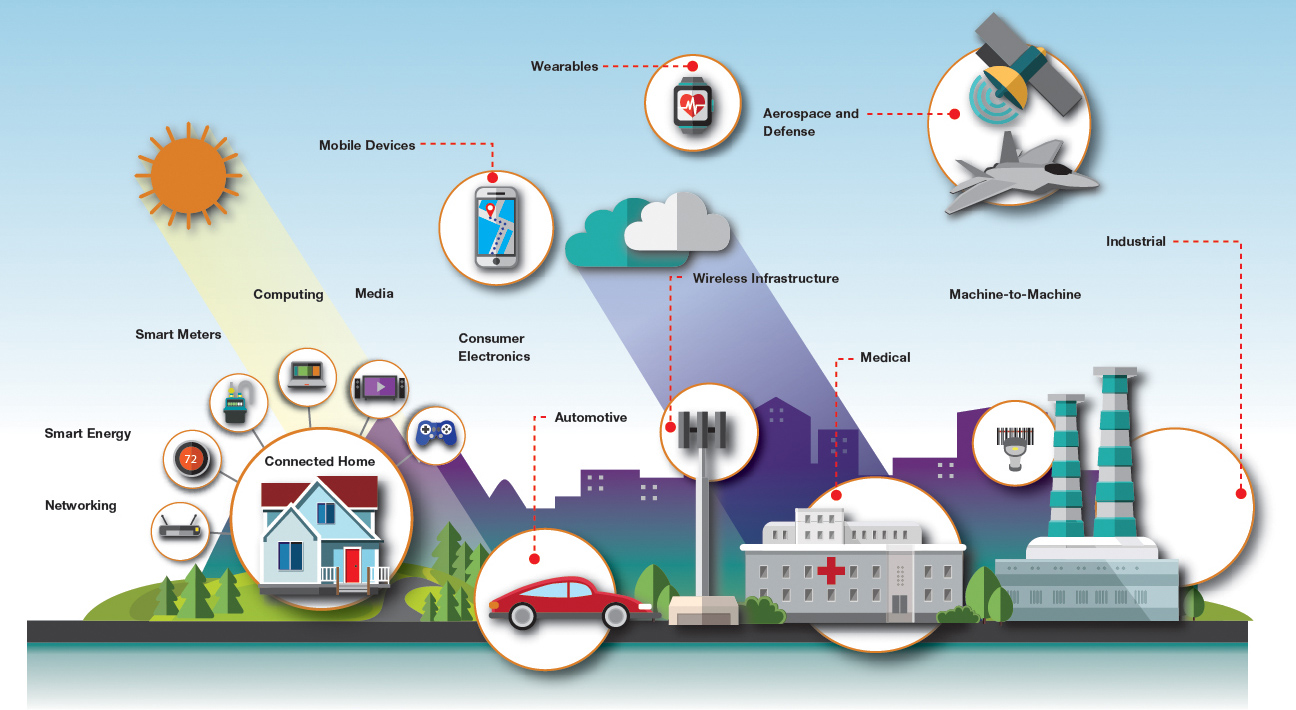
\includegraphics[scale=0.25]{images/broucer}
	\end{figure}
\end{block}
}

%%%%%%%%%%%%%%%%%%%%%%%%%%%%%%%%%%%%%%%%%%%

\frame{\frametitle{}
	\centering
	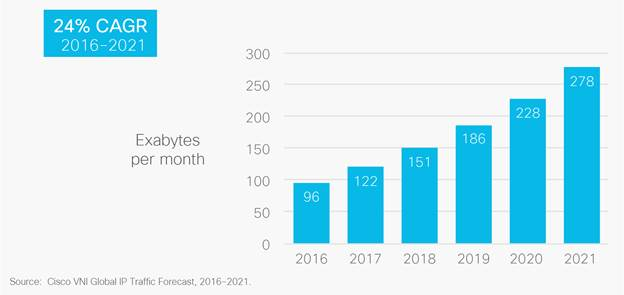
\includegraphics[width=8cm,height=4cm]{images/vni-hyperconnectivity-wp_0}
	\pause
	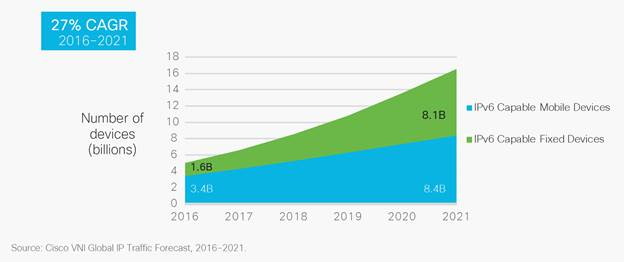
\includegraphics[width=8cm,height=4cm]{images/vni-hyperconnectivity-wp_7}
}

\frame{\frametitle{Need for Computational Power}
\begin{itemize}
	\item More data to process 
	\item Requirements for higher precision solvers
	
\end{itemize}
	\begin{figure}
	\centering
	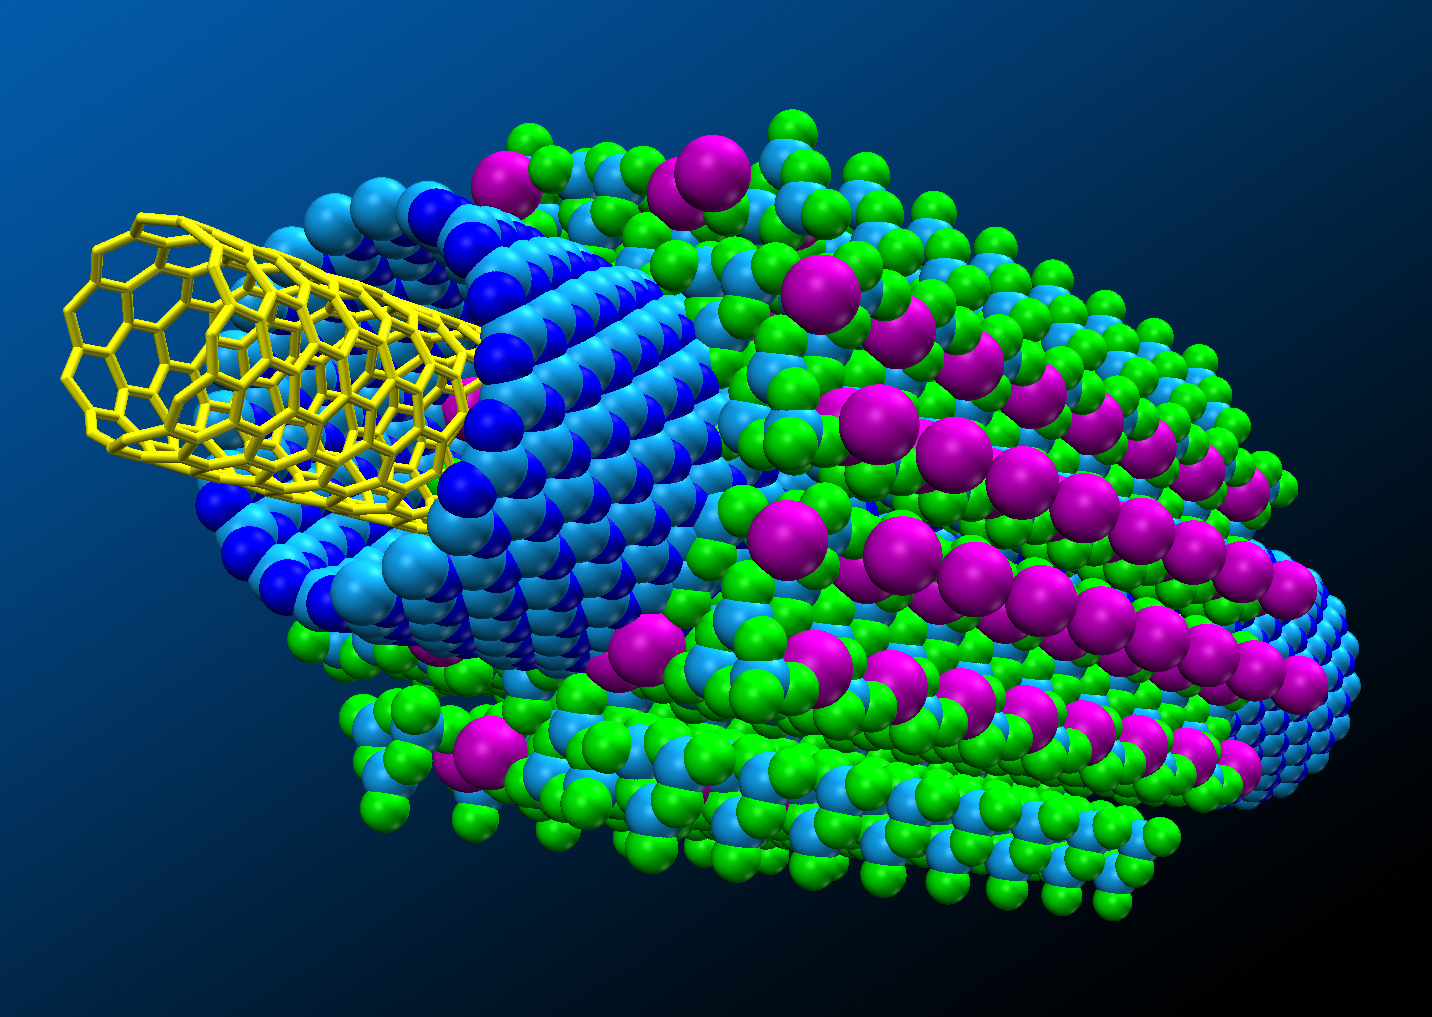
\includegraphics[width=0.8\textwidth]{images/material}
	\caption{Atomic Scale Material Simulation}
\end{figure}

}

%\frame{\frametitle{}
%	\centering
%	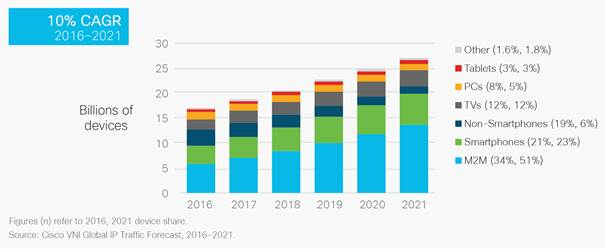
\includegraphics[width=8cm,height=4cm]{images/vni-hyperconnectivity-wp_2}
%	\pause
%	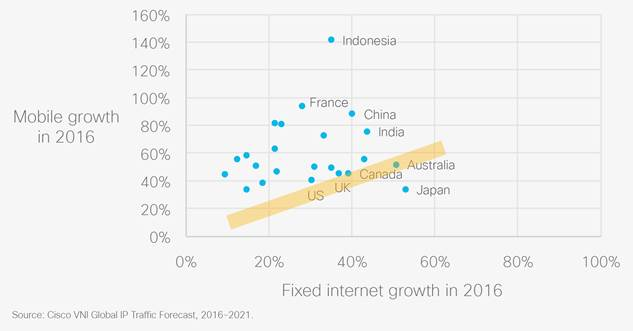
\includegraphics[width=8cm,height=4cm]{images/vni-hyperconnectivity-wp_1}
%}

\frame{\frametitle{Performance Improvements}
	\begin{center}
		\begin{block}{}
		 \begin{itemize}
		 	\item More Functional Units
		 	\item Higher Clock Speed
		 	\pause
		 	\item (A lot) More Transistor- Moore's Law
		 \end{itemize}
		\end{block}
	\end{center}
\begin{figure}
	\centering
	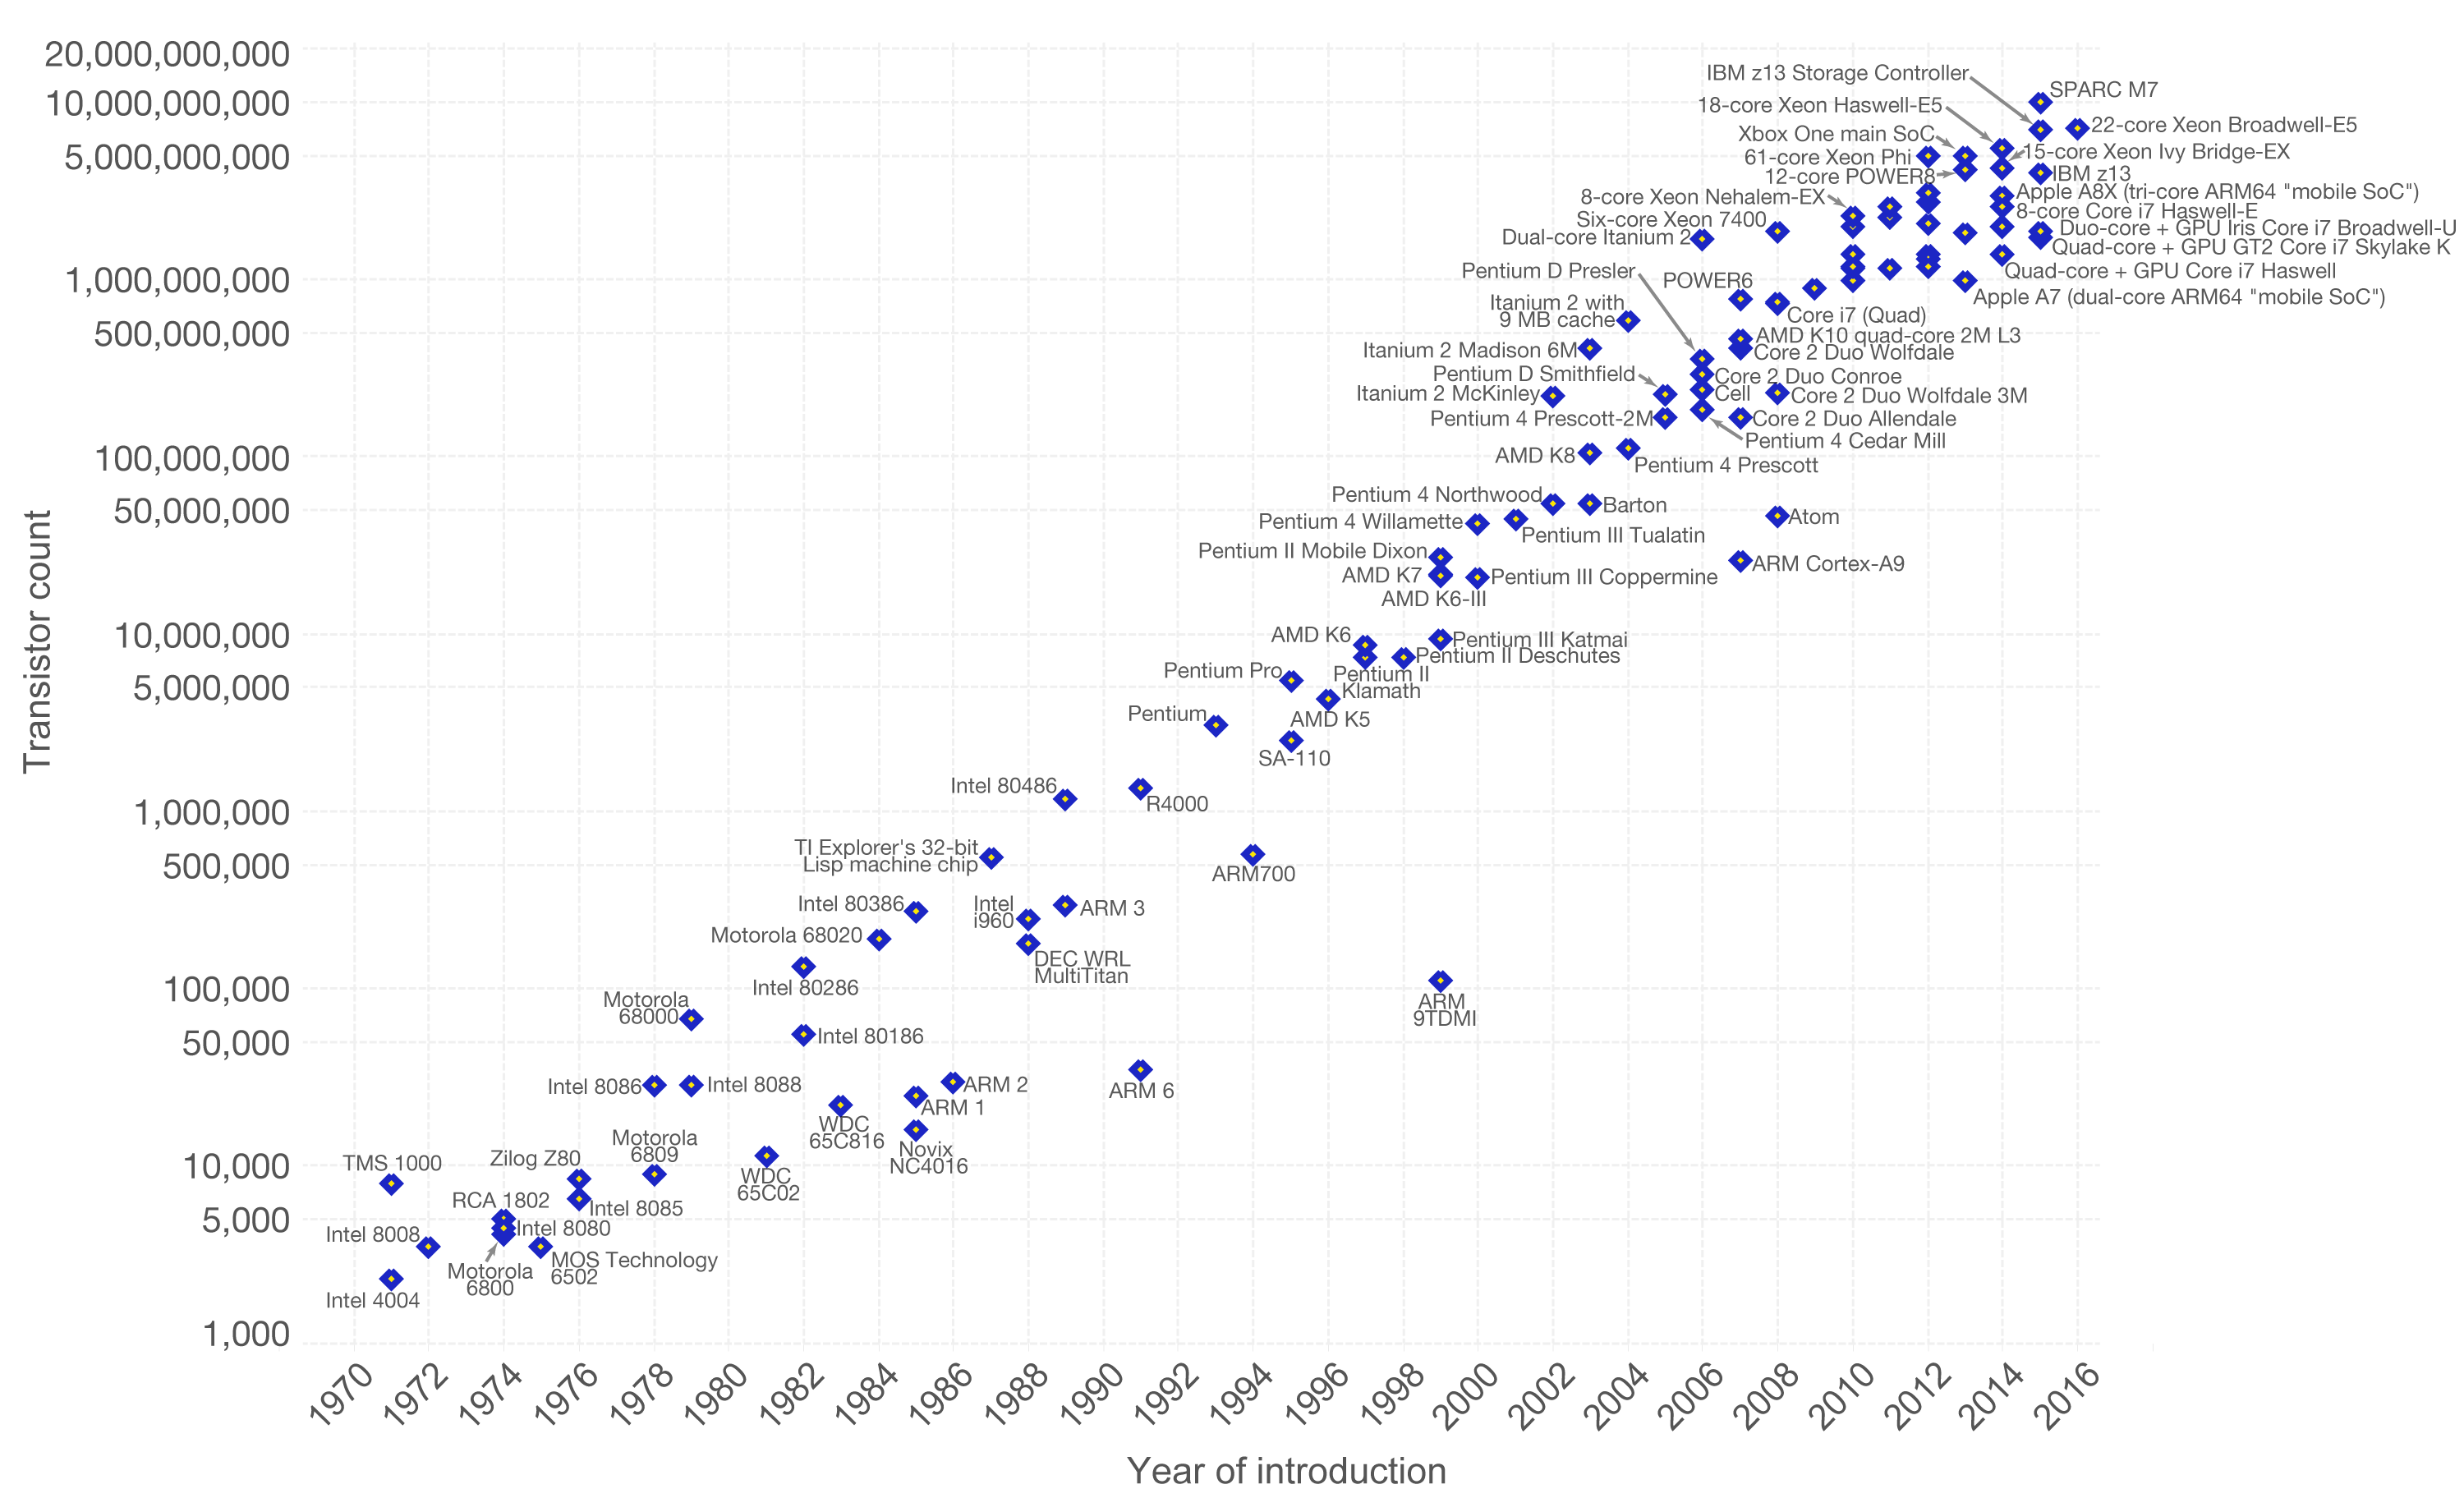
\includegraphics[width=0.8\textwidth]{images/moore_law2}
	\caption{Moore's law}
\end{figure}

}

%%%%%%%%%%%%%%%%%%%%%%%%%%%%%%%%%%%%%%%%%%%

\frame{\frametitle{This growth is not sustainable}
\centering
 Higher Clock and More Transistors = \textbf{More Heat}
 
\begin{figure}
	\centering
	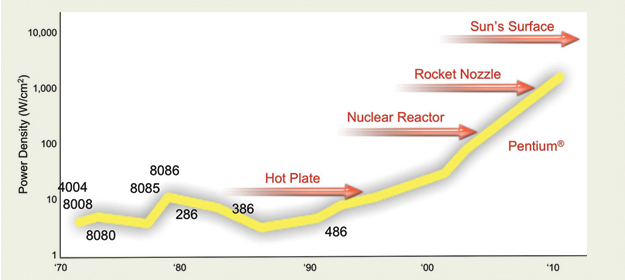
\includegraphics[width=\textwidth]{images/temperatureCPU}
\end{figure}
\pause
\begin{block}{Transistor size Limit} 
\begin{itemize}
	\item $7nm$ transistor is already possible
	\item $5nm$ will be in $4$ years
	\pause
	\item \textbf{Silicon atomic size is $0.2nm$}
\end{itemize}	
\end{block}

}

\frame{\frametitle{Parallelism}
		\begin{itemize}
			\item Computational power demans is increasing
			\item Parallelism is the answer
			\item Almost every device has multiple computing core: phone, cars, laptop etc.
			\item Especially true for dedicated computing machine
		\end{itemize}	
	
	\begin{figure}
		\centering
		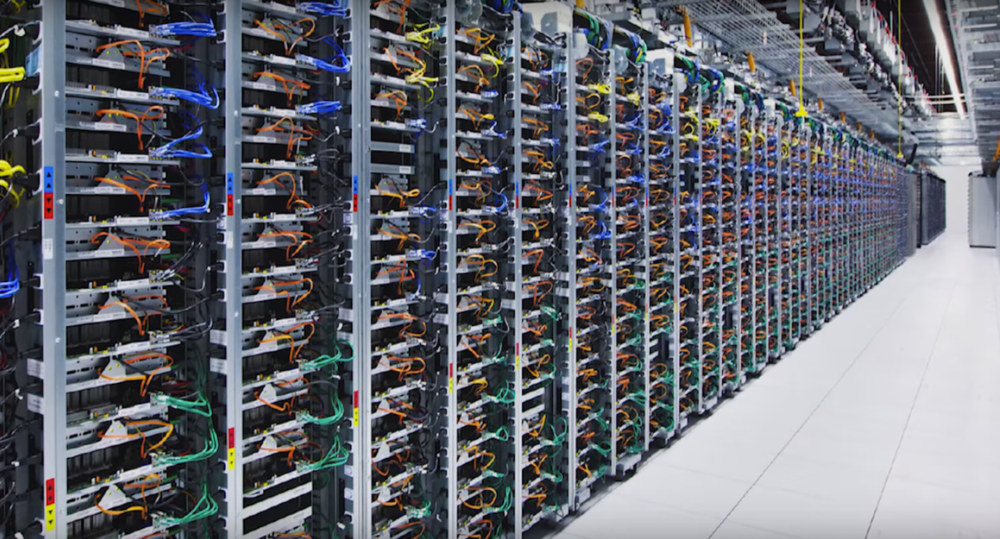
\includegraphics[width=\textwidth]{images/GoogleDataCenter}
	\end{figure}
}

\frame{\frametitle{Parallelism}
	\begin{block}{Trend in Scientific Computing HW}
		\begin{itemize}
			\item Large cluster of heterogeneous HW
			\item Heavy use of Accelerators (FPGA, Intel MIC, GPUs)
			\item Programming this machine is \textbf{very} hard
			\item Especially true for non parallel computing specialist
			\item One needs to master low-level details in order to write efficient solvers for such HW
		\end{itemize}	
	\end{block}
\begin{block}{Programming heterogeneous HW}
	\begin{itemize}
		\item is \textbf{very} complex
		\item Especially true for non parallel computing specialist
		\item One needs to master low-level details in order to write efficient solvers for such HW
	\end{itemize}	
\end{block}


}

\frame{\frametitle{Scope of the Thesis}
	\centering
	\textbf{The main goal of my work} 
	
\begin{itemize}
	\item a software framework for
	\item writing efficient solvers for regular grid methods
	\item targeting heterogeneous HW
\end{itemize} 
		\begin{figure}
		\centering
		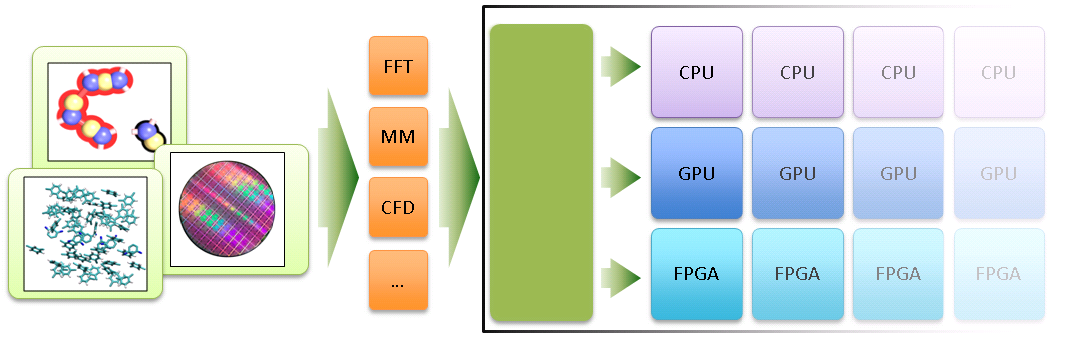
\includegraphics[width=\textwidth]{images/heterogen_modular_mapping}
	\end{figure}
}


%

